\section{Theoretischer Hintergrund}
\subsection{Maschinelles Lernen}
Maschinelles Lernen beschreibt das Konzept, auf Basis von einer großen Menge von Daten Algorithmen zu approximieren, die auf anderem Wege nicht erschlossen werden können. Man nehme beispielsweise die klassische Aufgabe, ein Programm zu schreiben, das in der Lage ist, Bilder von Hunden und Katzen zu unterscheiden. Wenn wir als Menschen uns dieser Aufgabe stellen, müssen wir nicht lange überlegen, wir lösen sie intuitiv. Wenn wir uns aber fragen, nach welchen Regeln wir diese Entscheidung treffen, wird es schon schwieriger. Wir könnten uns auf die Form der Ohren, die Farbe des Fells oder die Größe des Tieres konzentrieren. Aber wie genau wir Regelmäßigkeiten definieren, ist nicht so einfach. Maschinelles Lernen verfolgt den Ansatz, genau solche Regeln nicht mehr fest zu definieren, sondern sie anhand von einer großen Menge von Daten zu lernen \parencite[Vgl.][S. 2f.]{bishop_2006}.

\subsection{Neuronale Netze}
Ein Mittel der Wahl um das Konzept des maschinellen Lernens umzusetzen, sind sogenannte künstliche Neuronale Netze. Neuronale Netze, lose inspiriert von der Struktur des menschlichen Gehirns, bestehen aus einer Vielzahl von einfacher Einheiten, sogenannte Knoten, die in Schichten angeordnet sind und über unterschiedlich gewichtete Verbindungen verknüpft sind. Diese Struktur ermöglicht es, komplexe statistische Zusammenhänge in einem Datensatz zu modellieren, indem für einen gegebenen Datensatz mithilfe von Techniken des maschinellen Lernens die Parameter, also beispielsweise die Gewichte der Verbindungen des Netzes, so angepasst werden, dass sie die gegeben Daten möglichst genau abbilden. Wurde dieser Prozess erfolgreich durchlaufen, so kann das Modell im Anschluss dazu genutzt werden, Aussagen über Daten, die es im Lernprozess noch nie gesehen hat, zu treffen oder Vorhersagen abzugeben. Das interessante an diesem Ansatz ist es, dass durch diesen Ansatz, gerade bei großen neuronalen Netzen auch nicht triviale, subtile Muster im Datensatz erkannt werden können und so, wie oben bereits angedeutet, Approximationen für Probleme getroffen werden können, die formal nur schwer beschrieben werden können \parencite[Vgl.][S. 225f.]{bishop_2006}.

\subsection{Word Embeddings}
Eine weitere, für diese Arbeit relevante Entwicklung der jüngeren Forschung sind die Fortschritte der Computerlinguistik. Ein Kernproblem dieses Feldes ist die Forschung an der Repräsentationen von Sprache. Hierbei geht es nicht einfach darum, einzelne Wörter in ihrer Schriftform zu speichern, sondern vielmehr den Wort\emph{sinn} festzuhalten. Man betrachte zum Beispiel die Wörter \emph{Couch} und \emph{Sofa}, die in Schriftform, mit Ausnahme des zweiten Buchstabens vollkommen unterschiedlich sind, in ihrer Bedeutung aber nahezu Synonym verwendet werden. Weiterhin möchten wir Aussagen über die Beziehung von Wörtern treffen können. \emph{Heiß} und \emph{kalt} haben in ihrer Wortbedeutung einen klaren Zusammenhang (Es handelt sich um Gegensätze), den wir eventuell darstellen möchten, genauso wie \emph{Replika} und \emph{Fälschung} im Grunde dasselbe meinen, aber einen klaren Unterschied in ihrer Konnotation aufweisen \parencite[Vgl.][S. 106ff.]{jurafsky_martin_2020}. 
Eine Form der semantisch reichen Repräsentationen zu finden, die diesen Anforderungen genügt ist nicht trivial, es handelt sich aber wieder um ein solches Problem, das, wie oben beschrieben, intuitiv einfach zu lösen, formal jedoch schwer zu beschreiben ist. Und genau wie oben beschrieben, können die Techniken aus dem Feld des maschinellen Lernens auf dieses Problem angewandt werden, um es zu lösen. \\

Die Grundlage für die nun folgenden Überlegungen bildet die 1950 erstmals formulierte Verteilungshypothese der Linguistik. Im Grunde besagt sie, dass Wörter, die in ähnlichen Kontexten auftauchen, eine ähnliche Bedeutung haben. Wenn die Wörter \emph{Pizza} und \emph{Burger} beispielsweise beide häufig im Zusammenhang mit den Wörtern \emph{Essen} und \emph{geniessen} auftauchen, kann daraus geschlossen werden, dass sie ihr Wortsinn eine Ähnlichkeit hat, in diesem Fall, dass es sich bei beiden Wörtern um Essen handelt. \parencite[Vgl.][S. 109]{jurafsky_martin_2020}\\

Auf Basis dieser Erkenntnis kann eine erste simple Repräsentationen des Wortsinns gefunden werden. Gegeben sei ein Corpus $C$ auf Basis dessen wir einen Wortsinn für jedes Wort im Vokabular $V$ des Corpus finden wollen. Auf Basis der Verteilungshypothese kann nun eine Wort-Wort-Matrix aufgestellt werden, die abbildet, wie häufig Worte im Kontext anderer Worte auftauchen. Dafür muss ein Kontext definiert werden, häufig ist dieser Kontext ein Bereich um das Wort, kann aber auch beliebig definiert werden, beispielsweise als eine Menge Dokumente im Corpus. Als Ergebnis erhält man eine Matrix mit der Dimension $ | V | \times | V | $, beziehungsweise einen $|V|$-dimensionalen Spaltenvektor für jedes Wort \parencite[Vgl. ][S. 113]{jurafsky_martin_2020}.\\

\begin{table}
    \centering
    \begin{tabular}{ | c | c | c | c | }
        \rowcolor{tableHeading} & Essen & italienisch & Auto \\
        Pizza & 150 & 122 & 11 \\
        Burger & 136 & 3 & 13 \\
        Porsche & 0 & 6 & 350 \\
        Ferrari & 1 & 199 & 475 \\
    \end{tabular}
    \label{Vector Semantics Word-Word Vec Table}
    \caption{Wort-Wort-Matrix auf Basis des Wikipedia Corpus und ausgewählten Worten \parencite{davies_2015}}
\end{table}
\begin{figure}[H]
    \tdplotsetmaincoords{70}{110}
    \begin{tikzpicture}[tdplot_main_coords,line cap=round,>=stealth]
    \draw (0,0,0) --  (14,0,0)  node[pos=1.1]{Auto};
    \draw (0,0,0) -- (0,6,0) node[pos=1.105]{Essen};
    \draw (0,0,0) -- (0,0,6) node[pos=1.05]{italienisch};

    \draw  (5,0,0) node[right]{$150$} -- ++ (0,0,0.15)
            (0,5,0) node[below]{$150$} -- ++ (0,0,0.15)
            (0,0,5) node[right]{$150$} -- ++ (0,-0.15,0);

    \draw[very thick,->=0.7, color=blue] (0,0,0)  -- (0.36,5,4.03) node[above]{Pizza};
    \draw[very thick,->=0.7, color=blue] (0,0,0)  -- (0.43,4.53,0.1) node[above]{Burger}; 
    \draw[very thick,->=0.7, color=blue] (0,0,0)  -- (11.66,0,0.2) node[left]{Porsche};
    \draw[very thick,->=0.7, color=blue] (0,0,0)  -- (15.83,0.03,6.63) node[above]{Ferrari};

    \end{tikzpicture}
    \caption{Visualisierung der in Tabelle \ref{Vector Semantics Word-Word Vec Table} berechneten Vektoren in dreidimsionalem Raum}
    \label{Vector Semantics Word-Word Vec}
\end{figure}
Die so gewonnen Vektoren haben bereits einige der gewünschte Eigenschaften um den Wortsinn zu encodieren. Die in Tabelle \ref{Vector Semantics Word-Word Vec Table} dargestellte Wort-Wort-Matrix basiert auf dem Corpus der englischsprachigen Wikipedia und illustriert eine Eigenschaft, die auch noch bei der Reduktion auf wenige Dimensionen sichtbar wird: Wörter, die sich ähnlich sind, tauchen in ähnlichen Kontexten auf. Die Vektoren für Automarken tauchen beide ähnlich häufig im Kontext des Wortes Auto auf, genauso wie Essbares ähnlich häufig im Kontext von dem Wort Essen auftauchen. Auch eine 1970 entwicklelte Methode zur Beschreibung von Analogieproblemen lässt sich anwenden. \parencite[Vgl.][]{RUMELHART19731} Die Idee dieser Methode ist es Fragen nach folgendem Schema zu stellen: \emph{Deutschland gehört zu Berlin. Was gehört zu Paris?} Auch bei diesem sehr simplifizierten Beispiel lässt sich ein solches Sinn-Parallelogram aufstellen. Anhand der in Abbildung \ref{Vector Semantics Word-Word Vec} getroffenen Visualisierung des Beispiels lässt sich leicht erkennen, dass dieses Problem durch einfach Vektorrechnung lösen lässt. \emph{Pizza gehört zu Burger. Was gehört zu Porsche?}. Die Antwort innerhalb dieses Beispiels ist Ferrari und lässt sich bestimmen, indem der Vektor für Pizza von Burger subtrahiert wird und das Ergebnis dieser Operation auf den Vektor für Porsche aufaddiert wird. Das Ergebnis ist ein Vektor der in die Nähe von Ferrari zeigt. Dieses Beispiel ist selbstverständlich enorm simplifiziert, es lässt sich aber genau diese Encodierung von Wortsinn auch bei größeren Vokabularien feststellen\footnote{Einer der wohl bekanntesten Beispiele aus diesem Feld ist der Erfolg aus dem word2vec paper, indem das Modell den Zusammenhang zwischen König minus Mann plus Frau ist gleich Königin herstellen konnte \parencite[Vgl.][]{mikolov_chen_corrado_dean_2013}.} \parencite[Vgl.][S. 128f.]{jurafsky_martin_2020}. \\

Vorgestellt wurde die hiermit die einfachste Form von statischen, also kontextunabhängige, Embeddings, mittlerweile gibt es eine Vielzahl von Techniken um dieses stumpfe Zählen von Worten mit verschiedenen Verfahren zu optimieren und schlussendlich bessere und sinnhaltigere Ergebnisse zu erzielen. Ein Problem dieser Methode ist beispielsweise, dass die so gewonnen Vektoren eine sehr hohe Dimensionalität haben ($|V|$), dafür aber größtenteils leer sind, man spricht von dünnbesetzten Vektoren. Die Empirik hat gezeigt, dass sich wesentlich bessere Ergebnisse erzielen lassen, wenn Wörter als Vektoren mit niedrigerer Dimensionalität dargestellt werden, also "dicht" sind. Die Intuition hinter dieser Erkenntnis ist es, dass dadurch eine gewisse "Abstraktion" des Wortsinnes stattfindet und so konzeptuelle Zusammenhänge besser abgebildet werden können. \parencite[Vgl.][S. 113f.]{jurafsky_martin_2020} \\

Ein großer Durchbruch bei diesem Problem wurde beispielsweise durch den Ansatz der Autoren des Word2Vec Papers erzielt, die ihrem Algorithmus \emph{Skip-Gram with negative sampling} ein statisches, aber dichtes Embedding berechnen. SGNS ist eine Methode, um Wort-Embeddings mithilfe von Techniken des maschinellen Lernens zu trainieren, indem ein Modell trainiert wird, das die Kontextwörter um ein Zielwort innerhalb eines Fensters vorhersagen soll, während gleichzeitig echte Kontextwörter von zufällig ausgewählten negativen Beispielen unterschieden werden. Das zu Grunde liegende statistische Modell wird dabei immer besser darin, gegeben ein Wort, zu bestimmen, ob ein anderes Wort wahrscheinlich ist in dessen Kontext aufzutauchen. Die eigentlichen Embeddings, die das Ziel dieses Vorgehens sind, sind dabei die Eingabe in den Algorithmus und werden solange angepasst, bis das Modell mit einer gewünschten Verlässlichkeit vorhersagen kann, ob die Eingabe ein echtes Kontextwort ist, oder nicht. \parencite[Vgl. ][]{mikolov_chen_corrado_dean_2013}.


\subsection{Text Embeddings und die Transformer Architektur}
Den bisher vorgestellen Methoden, um semantisch reiche Repräsentationen von Worten zu erstellen, fehlt ein entscheidendes Merkmal, um sie für praktisch nutzen zu können: Ihnen fehlt der Kontext. Bis jetzt haben wir immer ausschließlich versucht, einzelne Wörter in ihrer Bedeutung zu erfassen, ohne dabei auf den Kontext einzugehen, in dem sie auftreten. Ein Wort wie \emph{Bank} kann beispielsweise sowohl ein Möbelstück, als auch eine Finanzinstitution beschreiben. Die Bedeutung des Wortes hängt also stark vom Kontext ab. Für die letztendliche Anwendung ist das insofern relevant, als dass bei der Analyse von Geschäftsdaten immer gesamte Dokumente von Bedeutung sind. Was bringt es mir, wenn ich die Bedeutung einzelner Wörter in der Beschreibung eines Bauteils kenne, nicht aber ihren Zusammenhang untereinander? \\

Es muss also eine Methode gefunden werden, Embeddings nicht auf einzelnen Wörtern zu erstellen, sondern ganze Texte zu verarbeiten. Der aktuelle Stand der Technik ist dabei die Transformer Architektur. Hierbei handelt sich auch um die Technik, die Anfang 2021 von OpenAI in Form von ChatGPT zu weltweiter Bekanntheit gelangt ist. Die Grundidee dieser Architektur ist es, über eine Reihe von sogenannten Transformer-Blöcken graduell die Eingabewörter mit ihrem Kontext anzureichern. \\

\begin{figure}[H]
    \centering
    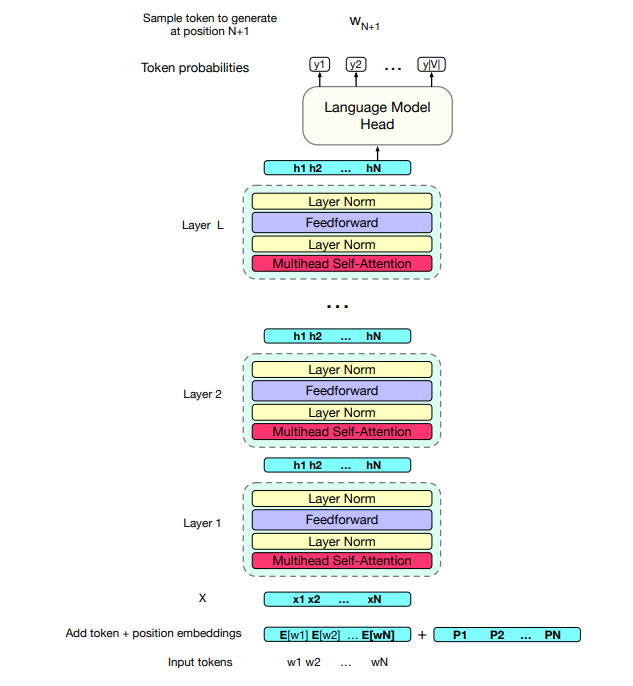
\includegraphics[width=1\textwidth]{Transformer-Architektur.png}
    \caption{Die Architektur eines Transformers für die Anwendung als Sprachmodell \parencite{jurafsky_martin_2020}}
    \label{Transformer}
\end{figure}

Die in Abbildung \ref{Transformer} dargestellte Architektur zeigt den Aufbau eines solchen Transformers. An Anfang des Modells stehen die Eingabe-Embeddings. Ähnlich der Word-Embeddings der Word2Vec Algorithmus handelt es sich hierbei um dichte Vektoren, die im Rahmen des Training des Modells erlernt werden und einzelne Wörter darstellen.\footnote{Es bleibt anzumerken, dass diese Word-Embeddings sich in den meisten Fällen nicht mehr auf Wörter im Sinne der Sprache beziehen, sondern der zugrundeliegende Corpus algorithmisch in kleinste Einheiten zerlegt wird. Diese Einheiten werden häufig auch als Tokens bezeichnet. } Das interessante an der Transformer-Architektur ist es nun aber, dass sie ein sogenanntes Kontext-Fenster betrachtet, also einen kleinen Teilausschnitt aus dem Trainings-Corpus, um ein Wort eben nicht statisch, sondern im Kontext seiner direkten Nachbarn zu betrachten. Der entscheidende Innovation dabei ist, dass beim Transformer auch die Position und nicht einfach nur die Häufigkeit des nebeneinander Auftretens einbezogen wird. Um das zu erreichen, werden die Word Embeddings des Kontextfensters mit sogenannten Positions-Embeddings angereichert. Ein Positions-Embedding kann dabei wieder ein gelernter Vektor für jede Position im Kontextfenster sein oder auch eine simple Funktion, die beispielsweise durch eine Kombination von Sinus- und Kosinusfunktionen einer Position einen Vektor zuordnet.\footnote{Es gibt durchaus noch weitere Techniken, die Position eines Wortes als Embedding darzustellen, beispielsweise als relative Position zum betrachteten Wort, das soll in dieser Arbeit aber kein Thema sein. } Diese Eingabe wird nun in einem vielschichtigen neuronalen Netz verarbeitet, welches aus einer Reihe aus unterschiedlichen Komponenten besteht. Die interessanteste Komponente ist dabei wahrscheinlich der Multihead-Self-Attention Block.\\

\begin{figure}[H]
    \centering
    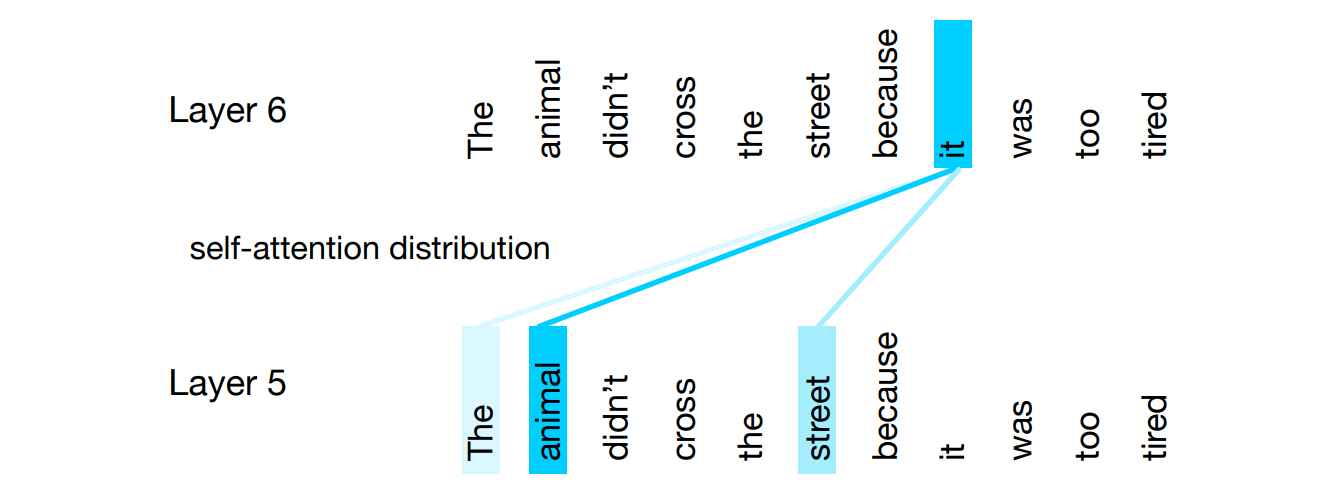
\includegraphics[width=1\textwidth]{Self Attention.png}
    \caption{Darstellung der Funktionsweise von Self Attention in einem Transformer}
    \label{SelfAttention}
\end{figure}

Self-Attention, oder Selbstaufmerksamkeit, ist eine Technik, die Eingaben im Modell miteinander zu verknüpfen. Bisher haben wir als Eingabe die Wörter des Kontextfensters voneinander getrennt betrachtet, jetzt soll durch Selbstaufmerksamkeit ein Verständnis für die Beziehungen zwischen den Eingaben gelernt werden. Das bedeutet, dass das Modell kontextuelle Beziehungen zwischen den Wörtern lernt, abhängig von deren Position im Satz. In der Abbildung \ref{SelfAttention} sehen wir ein Beispiel der Selbstaufmerksamkeitsverteilung zwischen den Wörtern "animal" und "it".\\

Im Grunde ist die Idee von Selbstaufmerksamkeit, für jedes Wort eine gewichtete Summe aller anderen Wortvektoren zu berechnen, wobei die Gewichte durch sogenannte Aufmerksamkeits-Scores bestimmt werden. Diese Scores werden durch das Skalarprodukt der Query- und Key-Vektoren der Wörter berechnet und anschließend normalisiert. In der Abbildung sehen wir, dass im Layer 5 der Transformer-Architektur das Wort "animal" eine hohe Aufmerksamkeit auf das Wort "it" im Layer 6 legt, was durch die blauen Linien dargestellt wird. Dies zeigt, dass das Modell die Beziehung zwischen "animal" und "it" erlernt hat, nämlich dass "it" sich auf "animal" bezieht. Der Vektor für "it" in Layer 6 berechnet sich nun aus einer gewichteten Summe aller Vektoren in Layer 5, wobei das Wort Animal besonders mit einbezogen wird. Indem viele dieser Selbstaufmerksamkeits-Blöcke hintereinander geschaltet werden, wird nach und nach aus den ursprünglichen Word Embeddings eine Reihe von kontextuell angereicherten Vektoren, die zusammengenommen den Sinn, der im Kontextfenster transportiert wird, abbilden können.\footnote{Dies ist natürlich eine einigermaßen vereinfachte Darstellung des Attention Mechanismus in modernen Sprachmodellen. Beispielsweise erweitert Multihead Attention die Idee der Self-Attention, indem er mehrere Selbstaufmerksamkeits-Layer (oder "Köpfe") parallel verwendet. Jeder dieser Köpfe lernt unterschiedliche Aspekte der Beziehungen zwischen den Wörtern. Die Eingabevektoren werden also in mehrere Teile aufgeteilt, und jede Teilmenge wird in einem separaten Selbstaufmerksamkeits-Layer verarbeitet. Jeder Kopf führt eine eigene Selbstaufmerksamkeitsoperation durch und erzeugt dabei eine eigene gewichtete Summe und Die Ergebnisse aller Köpfe werden dann zusammengeführt und in einen endgültigen Vektor integriert. Das aber nur am Rande.} \\

Wie bereits erwähnt ist Selbstaufmerksamkeit nicht die einzige Komponente, die in modernen Transformer-Architekturen eingesetzt wird, neben dieser Techniken spielen noch einfache Feed-Forward Layer, Residualverbindungen und Normalisierungen eine Rolle. Für den Zweck dieser Arbeit ist jedoch vor Allem relevant, dass der Transformer basierend auf einem Kontextfenster eine Reihe von kontextuell und semantisch angereicherten, dichten Vektoren produziert. Diese Embeddings erfassen den Sinn des eingegeben Text und werden somit als Text-Embeddings bezeichnet. In typischen Anwendungen dieser Modelle wird aus der Menge von Vektoren einer ausgewählt und als Repräsentationen des Textes verwendet.\footnote{Teilweise sind das extra für diesen Zweck eingefügte Tokens, in anderen Fällen der letzte Token. Die Intuition hinter der Technik ist es, dass durch Anwendung der Selbstaufmerksamkeit, der Sinn der im Kontext-Fenster transportiert wird, nach Anwendung des Verfahrens in jedem Token encodiert ist. } Das Ergebnis ist also ein Vektor, der den Sinn der Eingabe transportiert. Warum diese Embeddings so wertvoll sind, soll im nächsten Abschnitt in ihrer Anwendung geklärt werden.

\subsection{Ähnlichkeitssuche}
Wie bereits in der Einführung des Konzepts der Word Embeddings angedeutet, ist eine der zentralen Anwendungen von semantisch reichen Repräsentationen von Texten die Ähnlichkeitssuche. Die Idee dahinter ist es, dass semantisch ähnliche Texte auch ähnliche Embeddings haben. Daraus resultiert, dass es möglich wird, unstrukturierte Daten, wie es Texte sind, in einem strukturierten Raum zu repräsentieren und diese zu durchsuchen. Als Beispiel soll wieder der Corpus des englischsprachigen Wikipedia dienen. Berechnet man mithilfe der oben beschriebenen Methoden die Text-Embeddings für alle Artikel, erhält man eine Menge von Vektoren, die den Sinn der Artikel repräsentieren. Neben der Analyse des Datensatzes auf semantische Zusammenhänge und Themengruppen, ist die wahrscheinlich interessanteste Anwendung dieser Vektoren die Ähnlichkeitssuche. Hierzu wird eine Benutzeranfrage, nicht wie in typischen Suchsystemen auf Übereinstimmungen mit den Suchbegriffen oder vordefinierte Filtermöglichkeiten geprüft, sondern auf semantische Ähnlichkeit. Im Grunde wird also die Suchanfrage selbst in ein Embedding umgewandelt und schließlich mit den Embeddings der Dokumente verglichen. Zurückgegeben werden nun diejenigen Dokumente, die eine gewisse semantische Ähnlichkeit aufweisen, also inhaltlich die Anfrage des Benutzers beantworten. \\

\begin{figure}[H]
    \centering
    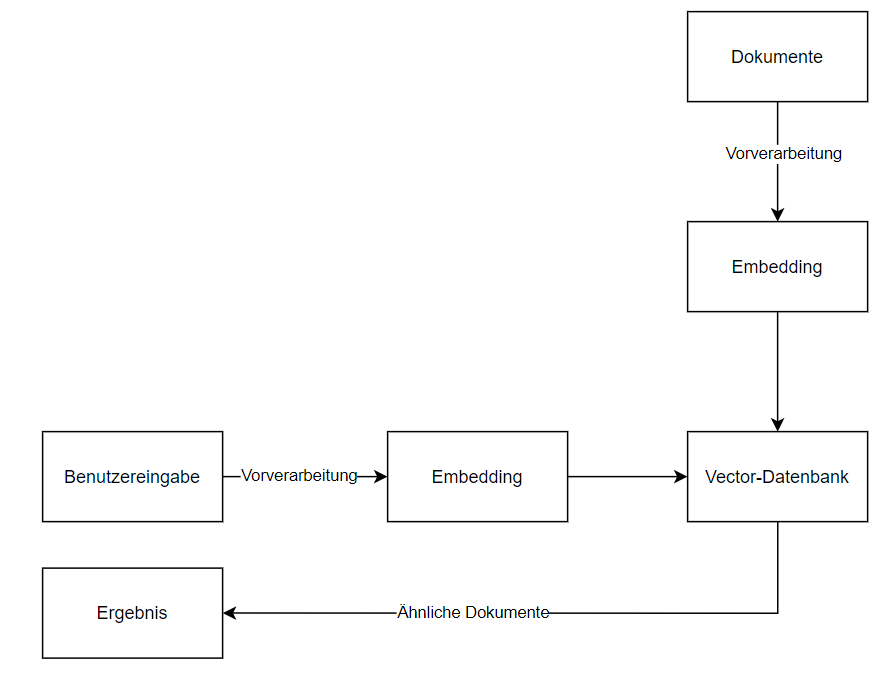
\includegraphics[width=1\textwidth]{Similarity Search.png}
    \caption{Darstellung der Architektur einer Ähnlichkeitssuche}
    \label{SimilaritySearch}
\end{figure}

In Abbildung \ref{SimilaritySearch} sehen wir ein Beispiel für die Architektur einer solchen Ähnlichkeitssuche. Ein Beispiel: Die Grundlage des Systems bildet eine Vektor-Datenbank, in der für jeden Artikel des englischsprachigen Wikipedia-Corpus ein Text-Embedding gespeichert ist. Diese Embeddings wurden im Vorfeld generiert, und verwenden als Eingabe vorverarbeitete Versionen der Wikipedia-Artikel, beispielsweise sind Bilder, Links und sonstige HTML-Elemente entfernt, sodass nur der Rohtext bleibt. Der Benutzer gibt die Anfrage "Was ist die Hauptstadt von Deutschland?" ein. Auch diese Eingabe wird vorverarbeitet. Beispielsweise muss sie zuerst übersetzt werden, da in der Datenbank englischsprachige Embeddings vorliegen. Nun wird die Anfrage in ein Text-Embedding umgewandelt und mit den Embeddings aller Dokumente im Corpus verglichen. Das geschieht mit Hilfe der Kosinus Ähnlichkeit, die als Maß der Ähnlichkeit zwischen zwei Vektoren den Winkel zwischen diesen anlegt. Die Dokumente, die die höchste semantische Ähnlichkeit aufweisen, werden schließlich zurückgegeben. Im Beispiel sind das die Artikel "Capital of Germany", "Berlin" und "Munich". Das bemerkenswerte an dieser Suche ist es, dass in der Eingabe an keiner Stelle die Rede von Berlin war, aber über die semantische Ähnlichkeit des Artikels "Berlin" zu der Eingabe "Hauptstadt" und "Deutschland" kann das richtige Ergebnis ermittelt werden. In einer klassischen Suche wäre wahrscheinlich das Ergebnis "Germany" oder "Capital" höher bewertet worden, da hier direkte Treffer im Titel des Artikels vorliegen. Stattdessen taucht aber München als Hauptstadt von Bayern in den Ergebnissen an dritter Stelle auf.\footnote{Dieses Beispiel ist nachzuvollziehen unter https://huggingface.co/spaces/abokbot/wikipedia-search-engine, mit der Eingabe "What is the capital city of Germany?"}

\subsection{Retrieval Augmented Generation}
Eine besondere Verwendung der oben besprochenen Ähnlichkeitssuche ist Retrieval Augmented Generation. Hierbei handelt es sich um eine Technik, die eingesetzt wird, um generativen Sprachmodellen zusätzliche Informationen zur Verfügung zu stellen, die sie beim Generieren von Sprache verwenden können. Bleiben wir beim Beispiel des Wikipedia-Datensatzes. Gegeben, es soll ein Chatbot auf Basis künstlicher Intelligenz entwickelt werden, der in der Lage ist, Fragen zu beantworten. Der klassische Transformer, wie er oben in seinen Grundzügen beschrieben ist, beherrscht diese Aufgabe bereits sehr gut. Limitiert ist er jedoch in seiner Fähigkeit, Quellen- und Fakten-basiert auf Fragen zu antworten. So antwortet er auf die Frage: ``Wer ist der Bundeskanzler von Deutschland?'' wahrscheinlich richtig mit ``Olaf Scholz'', er zieht diese Informationen jedoch aus seinem Trainingskorpus, seiner ``vor-trainierten, parametrischen Erinnerung'' \parencite[S. 2]{DBLP:journals/corr/abs-2005-11401}, nicht aus einer externen Quelle, also einer ``nicht-parametrischen Erinnerung''\footnote{\cite{DBLP:journals/corr/abs-2005-11401} meint mit diesem Ausdruck, dass das Modell ``Erinnerung'' im Trainingsprozess aufbaut, indem es bereits gesehenen Text in seinen Parametern encodiert.} \parencite[S. 2]{DBLP:journals/corr/abs-2005-11401}. Das bedeutet, sollte sich der Bundeskanzler ändern, würde der Chatbot weiterhin "Olaf Scholz" antworten, bis sich seine Trainingsdaten aktualisiert haben. In der Realität bietet sich dieses Problem durchaus, sei es bei der Interaktion mit tagesaktuellen Nachrichten, technischer Dokumentation oder betriebsinternen Quellen, die eventuell aus datenschutzrechtlichen Gründen nicht in einen Trainingskorpus überführt werden sollen. \\

Hier kommt RAG zur Hilfe. Die Idee hinter RAG ist es, dem Chatbot eine zusätzliche Komponente vorzuschalten, die, wie oben beschrieben, eine Ähnlichkeitssuche durchführt. Im Vorfeld wurden also alle relevanten Quellen in ein Embedding umgewandelt und in einer Vektor-Datenbank gespeichert. Die Anfrage des Nutzers ``Wer ist der Bundeskanzler von Deutschland?'' wird nun in ein Text-Embedding umgewandelt und mit den Embeddings der Quellen verglichen. Das Ergebnis ist eine Liste von Dokumenten, die die höchste semantische Ähnlichkeit aufweisen. Bevor dem Sprachmodell die Anfrage gestellt wird, wird nun die Antwort aus den Dokumenten extrahiert und dem Modell als zusätzliche Information zur Verfügung gestellt. Das Modell erhält also eine Anfrage nach dem Muster: ``Kontext: Der aktuelle Bundeskanzler der Bundesrepublik Deutschland ist Olaf Scholz. Frage: Wer ist der Bundeskanzler von Deutschland?'', und muss das Ergebnis nur noch als natürlichsprachliche Antwort generieren. Die Empirik hat gezeigt, dass gerade bei Aufgaben, die faktisches Wissen benötigen, RAG-Modelle gegenüber klassischen Sprachmodellen weitaus bessere Leistungen erbringen. \parencite[Vgl. ][]{DBLP:journals/corr/abs-2005-11401}